\documentclass[12pt,tikz,border=10pt]{standalone}
\usetikzlibrary{arrows.meta, positioning, calc}
\usepackage{amsmath}
\usepackage{amssymb}

\begin{document}
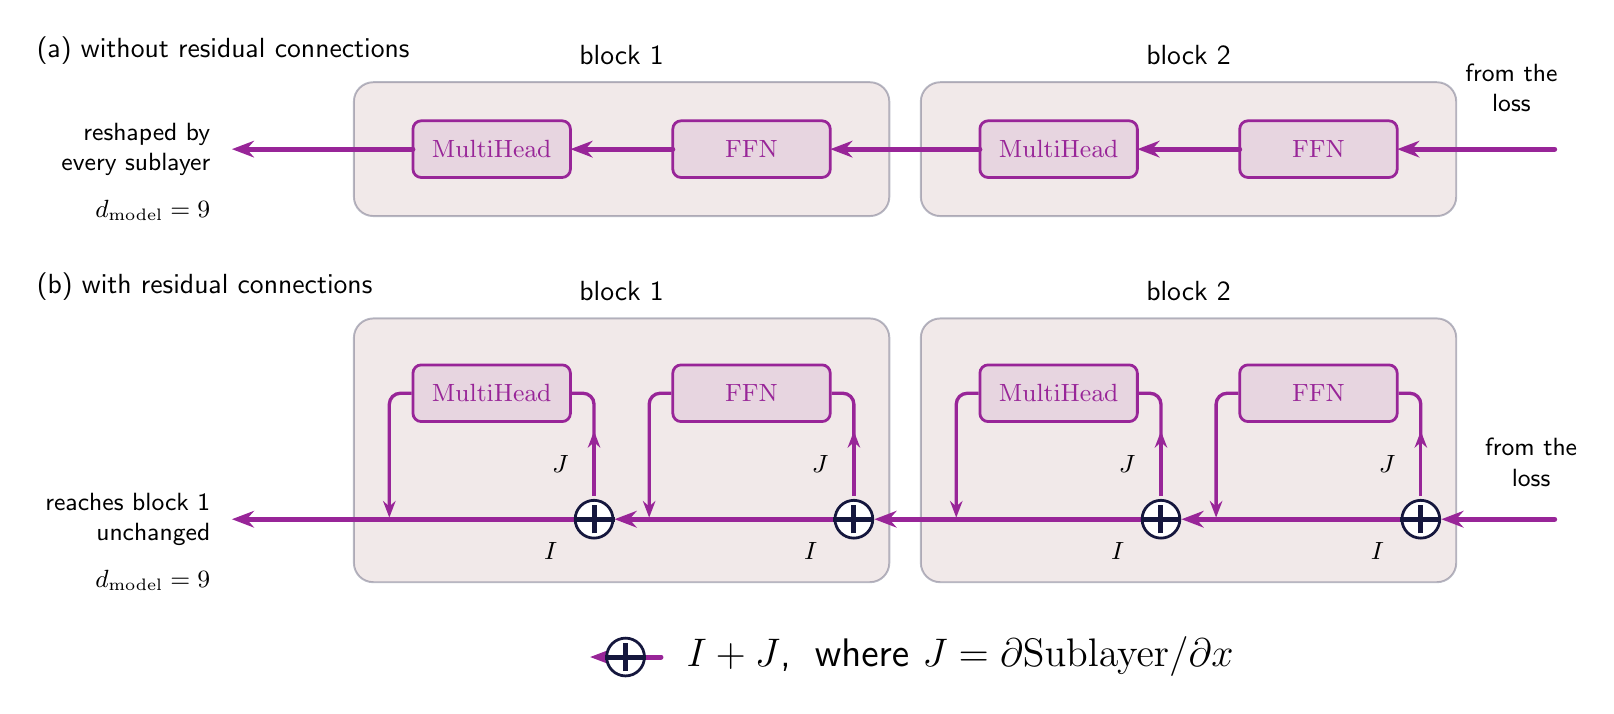
\begin{tikzpicture}[
    every node/.style={font=\sffamily},
]

\definecolor{c1}{HTML}{15173D}
\definecolor{c2}{HTML}{982598}
\definecolor{c3}{HTML}{E491C9}
\definecolor{c4}{HTML}{F1E9E9}
\definecolor{axiscolor}{HTML}{333333}
\definecolor{labelcolor}{HTML}{000000}

% ================================================================
%  GEOMETRY, planned before any TikZ was written.
%
%  The backward counterpart of residual_stream: same skeleton, same
%  pitch, same \addsym, but every arrowhead points LEFT.  Two rows
%  over the same two blocks; row (a) on top, row (b) below.
%
%  Shared x, residual_stream's numbers shifted +1.2 to open a left
%  margin for the row headers and the arrival labels:
%     block 1 at bx = 2.6, block 2 at bx = 9.8   (pitch 7.2)
%     panels  [bx-0.45, bx+6.35] -> [2.15,8.95] and [9.35,16.15]
%     titles centred at bx+2.95 -> 5.55 and 12.75
%     stream head (left, arrival) x = 0.6, tail (right) x = 17.4
%     sublayer x centres  3.9, 7.2, 11.1, 14.4   in BOTH rows, so the
%       two rows are column-for-column comparable
%
%  ROW (b), yshift 0, geometry lifted from residual_stream:
%     stream y = 0, sublayers ABOVE it, boxes 2.0 x 0.72 at y = 1.6
%     taps T in {2.6, 5.9, 9.8, 13.1}, adds A = T + 2.6
%         -> A in {5.2, 8.5, 12.4, 15.7}, box centre = T + 1.3
%     panel y [-0.8, 2.55] (raised 0.15 over residual_stream to seat
%         the dSublayer/dx label above the block-2 FFN box), title 2.65
%     backward stream: c2 at 1.8pt, one left arrow per segment,
%         tail A_right-0.26, head A_left+0.26 (the \addsym disc edge)
%     backward branch: c2 at 1.2pt, (A,0.30) up, left into box.east;
%         the riser carries an up head right at the split, the hook into
%         box.east is plain so no head is crushed into the 0.3 corner;
%         box.west, left to (T,1.6), down to (T,0.02) where it merges
%     I labels sit just left of each disc at (A-0.55, -0.40)
%     dSublayer/dx once, above the block-2 FFN box, anchor south 2.06
%
%  ROW (a), yshift 4.7: identical column centres, but the boxes sit ON
%     the stream at y = 0, so the single c2 arrow has to enter every
%     box's east side and leave its west.  No disc, no branch, no split.
%     panel y [-0.85, 0.85], title 0.95.
%
%  Ends, both rows: two-line arrival label anchored east at (0.45, 0)
%     with the width stamp under it at (0.45, -0.52); "from the loss"
%     two lines centred at (16.85, 0.78), clear of the last riser.
%  Row headers anchor south west at (-2.0, title y).
%  Key at y = -1.75, the same \addsym with a c2 backward stub.
%  Bounding box ~ [-2.0, 17.5] x [-2.0, 6.1]: 19.5cm wide, 8.1 tall.
% ================================================================

\tikzset{
  sub/.style={draw=c2, line width=1.0pt, fill=c2, fill opacity=0.10,
              text opacity=1, text=c2, rounded corners=3pt,
              minimum width=2.0cm, minimum height=0.72cm, inner sep=1pt,
              font=\sffamily\small},
  back/.style={-{Stealth[length=8pt]}, draw=c2, line width=1.8pt,
               line cap=round},
  bback/.style={-{Stealth[length=6pt]}, draw=c2, line width=1.2pt,
                rounded corners=4pt},
  panel/.style={fill=c4, rounded corners=7pt, draw=c1, draw opacity=0.30,
                line width=0.7pt},
  lab/.style={font=\sffamily\small, text=black},
  title/.style={font=\sffamily\normalsize, text=black, anchor=south},
  key/.style={font=\sffamily\Large, text=black},
}

% the residual add, exactly as in residual_stream
\newcommand{\addsym}[2]{%
  \fill[white] (#1, #2) circle (0.24);
  \draw[draw=c1, line width=1.0pt] (#1, #2) circle (0.24);
  \draw[draw=c1, line width=1.8pt] ({#1-0.26}, #2) -- ({#1+0.26}, #2);
  \draw[draw=c1, line width=1.8pt] (#1, {#2-0.18}) -- (#1, {#2+0.18});
}

% ================================================================
%  ROW (a)  no residual connections: the stream runs through the boxes
% ================================================================
\begin{scope}[yshift=4.7cm]

\foreach \bx/\b in {2.6/1, 9.8/2} {
    \draw[panel] ({\bx-0.45}, -0.85) rectangle ({\bx+6.35}, 0.85);
    \node[title] at ({\bx+2.95}, 0.95) {block \b};
}

\foreach \cx/\nm in {3.9/MultiHead, 7.2/FFN, 11.1/MultiHead, 14.4/FFN}
    { \node[sub] at (\cx, 0) {$\mathrm{\nm}$}; }

\foreach \ta/\he in {17.4/15.4, 13.4/12.1, 10.1/8.2, 6.2/4.9, 2.9/0.6}
    { \draw[back] (\ta, 0) -- (\he, 0); }

\node[title, anchor=south west] at (-2.0, 0.95)
    {(a) without residual connections};

\node[lab, anchor=east, align=right] at (0.45, 0)
    {reshaped by\\every sublayer};
\node[lab, anchor=north east] at (0.45, -0.52) {$d_{\mathrm{model}} = 9$};
\node[lab, align=center] at (16.85, 0.78) {from the\\loss};

\end{scope}

% ================================================================
%  ROW (b)  with residual connections: the stream is never interrupted
% ================================================================

\foreach \bx/\b in {2.6/1, 9.8/2} {
    \draw[panel] ({\bx-0.45}, -0.8) rectangle ({\bx+6.35}, 2.55);
    \node[title] at ({\bx+2.95}, 2.65) {block \b};
}

% the express lane: one left arrow per stretch between the adds
\foreach \ta/\he in {17.4/15.96, 15.44/12.66, 12.14/8.76, 8.24/5.46, 4.94/0.6}
    { \draw[back] (\ta, 0) -- (\he, 0); }

% the branch: up at the add, back through the sublayer, down at the tap
\foreach \bx/\b in {2.6/1, 9.8/2} {
    \foreach \t/\nm/\s in {0/MultiHead/m, 3.3/FFN/f} {
        \pgfmathsetmacro{\T}{\bx + \t}
        \pgfmathsetmacro{\A}{\T + 2.6}
        \node[sub] (\s\b) at ({\T + 1.3}, 1.6) {$\mathrm{\nm}$};
        \draw[bback] (\A, 0.30) -- (\A, 1.12);
        \draw[bback, -] (\A, 1.02) -- (\A, 1.6) -- (\s\b.east);
        \draw[bback] (\s\b.west) -- (\T, 1.6) -- (\T, 0.02);
        \node[lab] at ({\A - 0.55}, -0.40) {$I$};
        \node[lab, anchor=east] at ({\A - 0.20}, 0.70) {$J$};
    }
}

\foreach \a in {5.2, 8.5, 12.4, 15.7} { \addsym{\a}{0} }

\node[title, anchor=south west] at (-2.0, 2.65)
    {(b) with residual connections};

\node[lab, anchor=east, align=right] at (0.45, 0)
    {reaches block 1\\unchanged};
\node[lab, anchor=north east] at (0.45, -0.52) {$d_{\mathrm{model}} = 9$};
\node[lab, align=center] at (17.10, 0.72) {from the\\loss};

% ---------------------------------------------------------------- key
\draw[back] (6.05, -1.75) -- (5.15, -1.75);
\addsym{5.60}{-1.75}
\node[key, anchor=west] at (6.25, -1.75)
    {$I + J$,\; where $J = \partial\mathrm{Sublayer}/\partial x$};

\end{tikzpicture}
\end{document}
